
\section{processes.xml}

The process file is used to define cellular processes involved in
the production or degradation of macromolecules.

\subsection{RBAProcesses}
\label{sec:rba_processes}

The outermost portion of the process file is an instance of class
\rbaprocesses, shown in Figure~\ref{fig:processes_doc}.

\begin{figure}
  \centering
  
\includegraphics[scale=0.8]{figures/processes_doc}
  \caption{XML structure of process document.}
\label{fig:processes_doc}
\end{figure}

\rbamacromolecules{} has no simple attributes.
It contains exactly one instance of \textbf{ListOfProcesses}
and \textbf{ListOfProcessingMaps}.


\subsection{Process}
\label{sec:process}

The \process{} class is used to define cellular processes
(Fig.~\ref{fig:processes_process}).
Processes cover a wide variety of non-metabolic reactions.

\begin{figure}
  \centering
  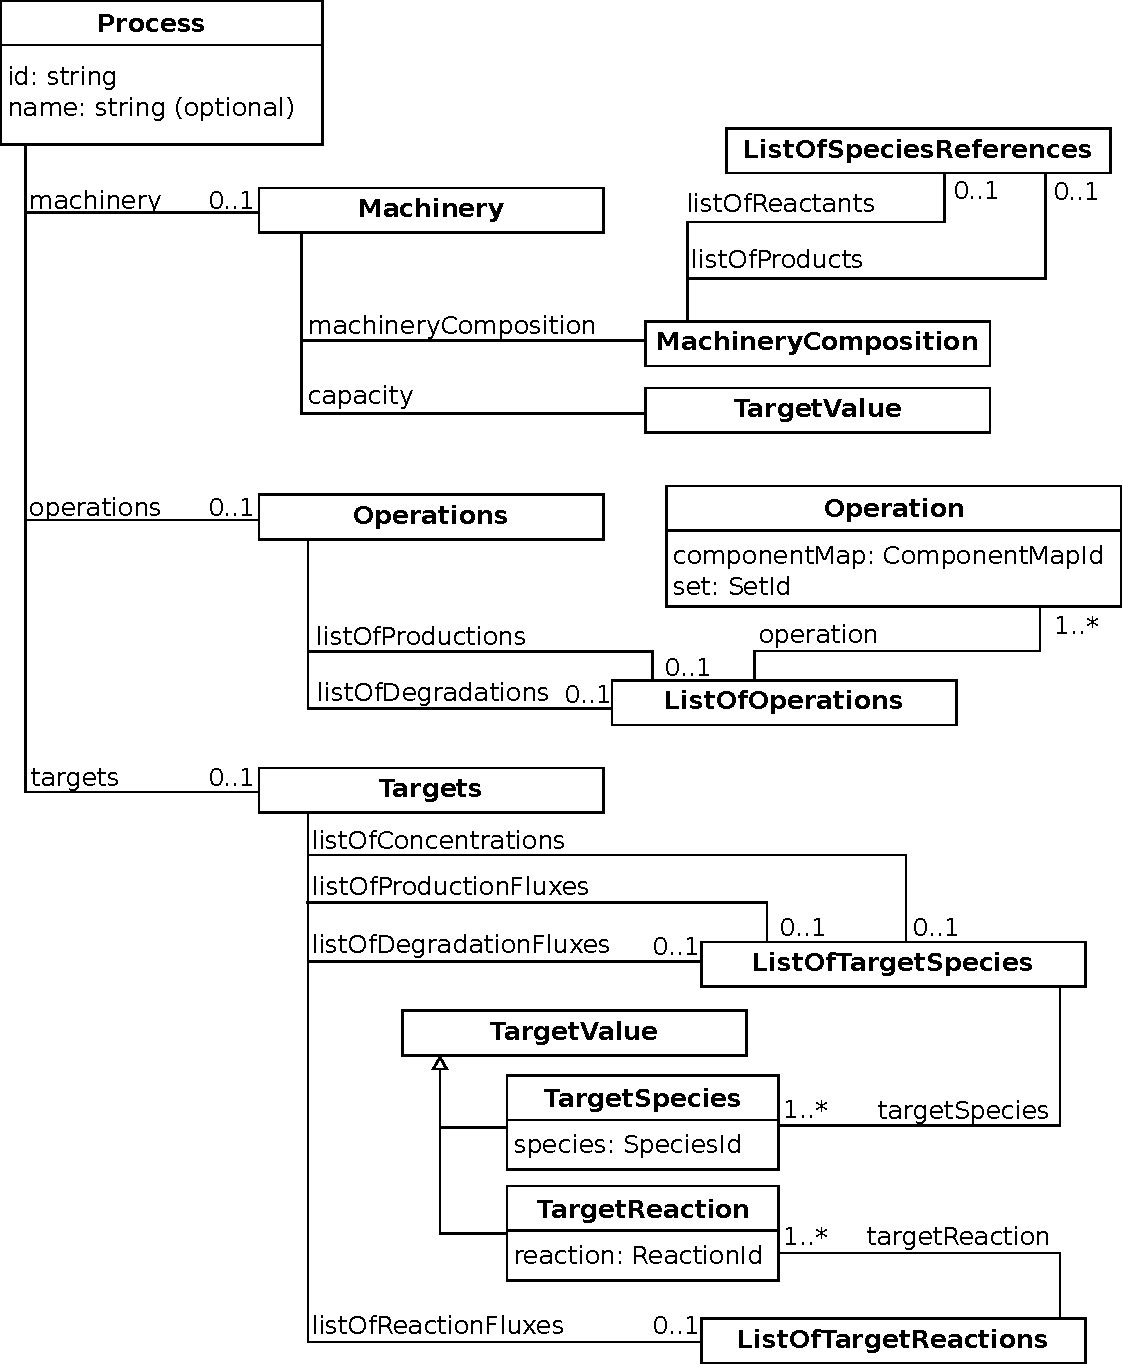
\includegraphics[scale=0.8]{figures/processes_process}
  \caption{Class used to store processes.}
\label{fig:processes_process}
\end{figure}

A \process{} revolves around 2 optional substructures.
The \machinery{} is the molecular entity enabling the process
(\textit{e.g.} ribosome for translation.)
Each machinery unit has a limited production/degradation capacity.
Every macromolecule produced by a process has a metabolite cost
(metabolites needed to produce/degrade it and byproducts).
However, if a machinery is defined, there is an additional cost
to produce the machinery that will enable the production/degradation of the
target.
This is similar to the production of \enzyme{}s in order to catalyze
metabolic \reaction{}s.

\processings{} define the sets of macromolecules that a process
produces or degrades.
The production reaction of a \macromolecule{} is determined by the \process{}es
it goes through.
For example, a protein's production reaction is defined by listing
the protein as an input in the \processings{} of the translation process.
If a protein is not listed as an input of any process, its production reaction
is empty, meaning that it does not cost anything to produce the protein.
\processings{} break down \macromolecule{}s in metabolic \species{}
and \machinery{} costs.

\paragraph{The \textit{id} attribute}
The \textbf{id} attribute is a string defining the identifier of a process.

\paragraph{The \textit{name} attirbute}
The \textbf{name} attribute is a string that can be used to give the process
a more human understandable name.


\subsection{Machinery}
\label{sec:machinery}

The \machinery{} class defines the machinery used by a process
(Fig.~\ref{fig:processes_process}).
\machinery{} has no simple attributes.
If a \machinery{} is defined, it defines a \emph{capacity constraint}.
Every \machinery{} unit is produced accordint to the reaction
defined by a \machinerycomposition.
Every unit also has a capacity defined by a \targetvalue.
The capacity defines how many targets a \machinery{} can process in 1 unit of
time.
Total capacity (base capacity multiplied by number of \machinery{} units)
must always exceed the number of targets produced.


\subsection{MachineryComposition}
\label{sec:machinery_composition}

The \machinerycomposition{} class defines the assembly costs of a complex
molecular machinery (Fig.~\ref{fig:processes_process}).
\machinerycomposition{} has no simple attributes.
It contains two \textbf{ListOfSpeciesReferences}.
One is for reactants, the other for byproducts of the assembly reaction.
Note that in this case, \speciesreference{}s can refer to \emph{both}
metabolic \species{} and \macromolecule{}s.
The assembly reaction should contain obvious components of the machinery,
but also metabolic costs related to assembly (such as ATP/GTP costs)
\emph{unless} these costs are already covered by a process.


\subsection{Processings}
\label{sec:processings}

The \processings{} relates \macromolecule{}s production/degradation to
some given \process{}es (Fig.~\ref{fig:processes_process}).
\processings{} has no simple attributes.
It may contain two \textbf{ListOfProcessings}, one for production and one for
degradation.


\subsection{Processing}
\label{sec:processing}

The \processing{} class defines how \macromolecule{}s are produced/degraded
(Fig.~\ref{fig:processes_process}).
\processing{} is used to break down \macromolecule{}s into metabolites
by linking them to a \processingmap.
It contains one \textbf{ListOfSpeciesReferences} that lists \macromolecule{}s
that are inputs of this process.
In this context, the species of a \speciesreference{} must be a macromolecule
and the stoichiometry attribute is ignored.

\paragraph{The \textit{processingMap} attribute}
The \textbf{processingMap} attribute must match the identifier of a
\processingmap.
This \processingmap{} will be used to compute the production/degradation
reaction of \macromolecule{}s, as well as \machinery{} costs.

\paragraph{The \textit{set} attribute}
The \textbf{set} attribute must refer to a \macromolecule{} set.
Currently, the only acceptable values are \textbf{protein}, \textbf{rna}
and \textbf{dna}.
\macromolecule{}s that are listed as input must belong to this set.


\subsection{ProcessingMap}
\label{sec:processing_map}

The \processingmap{} class is used to convert \macromolecule{}s in
metabolic and machinery costs (Fig.\ref{fig:processes_processing_map}).

\begin{figure}
  \centering
  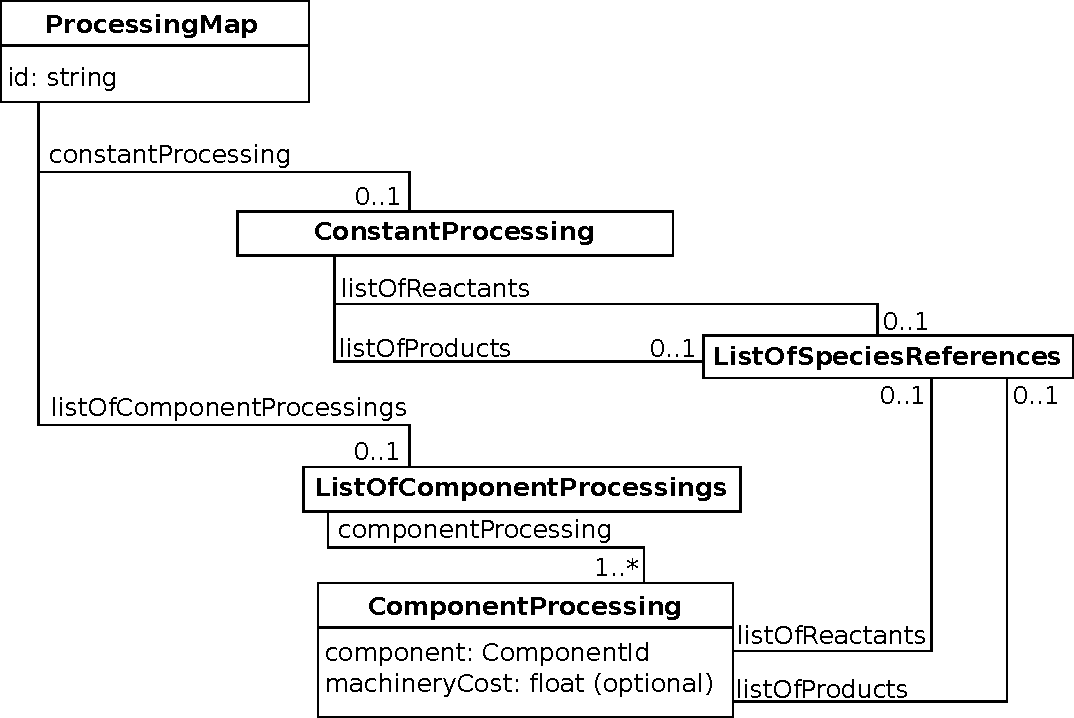
\includegraphics[scale=0.8]{figures/processes_processing_map}
  \caption{Class used to compute production/degradation of macromolecules.}
\label{fig:processes_processing_map}
\end{figure}

There are two types of processings.
The \constantprocessing{} lists metabolites that are always consumed or
produced when processing a macromolecule, no matter its composition
(\textit{e.g.} translation initiation).
The \textbf{ListOfComponentProcessing} container details
\componentprocessing{}s depending on the individual
\component{}s of the \macromolecule{}.
They cover metabolites used to assemble the \component{} onto the nascent
\macromolecule{}.
They also cover machinery costs, \textit{i.e.} how many \machinery{} units
are needed to assemble the \component{}.

\paragraph{The \textit{id} attribute}
The \textbf{id} attribute is a string defining the identifier of a
processing map.


\subsection{ConstantProcessing}
\label{sec:constant_processing}

The \constantprocessing{} class defines metabolites consumed and byproducts
generated by an assembly process (Fig.\ref{fig:processes_processing_map}).
It contains two \textbf{ListOfSpeciesReferences}, one for metabolites
consumed and one for metabolites produced.
Note that in this context, a \speciesreference{} must refer to a
metabolic \species.


\subsection{ComponentProcessing}
\label{sec:component_processing}

The \componentprocessing{} class defines metabolites consumed and byproducts
generated when assembling a specific \component{}
(Fig.\ref{fig:processes_processing_map}).
It contains two \textbf{ListOfSpeciesReferences}, one for metabolites
consumed and one for metabolites produced.
Note that in this context, a \speciesreference{} must refer to a
metabolic \species.
Additionally, it defines a machinery cost used in a \machinery{}'s
capacity constraint.

\paragraph{The \textit{component} attribute}
The \textbf{component} attribute is a string that must match the identifier
of a \component{}.

\paragraph{The \textit{machineryCost} attribute}
The \textbf{machineryCost} attribute is a real value that is used to
compute how many \machinery{} units are needed to assemble the \component{}.
For example, let the machinery cost for the processing of an amino acid be 1.
The capacity of the \machinery{} (the ribosome) is the number of amino acids
it can assemble per unit of time.
The machinery cost allows to compute how many ribosomes are needed
to produce the \component{} and, in the end, the \macromolecule{}
(in this example the number of amino acids divided by the ribosome's capacity).
